\chapter{Diseño\label{cap:disenho}}

En este capítulo se repasa el diseño de la aplicación a desarrollar.
Tras analizar los requisitos especificados en el capítulo \ref{cap:requisitos}, se ha decidido dividir la aplicación en dos partes, alojadas cada una en un servidor distinto: una interfaz web (\gls{front-end}) y un servicio web (\gls{back-end}).
Estos componentes están conectados por una red interna, y la comunicación entre ellos se realiza mediante llamadas  \gls{HTTP} (ver Figura \ref{fig:arquitectura}).

Esta arquitectura tiene una serie de ventajas respecto a tener todos los elementos del sistema en un mismo servidor físico.
En primer lugar, se sobrecarga menos el servidor de la sonda de red, minimizando así el impacto que la aplicación pueda tener sobre el rendimiento de la captura y reproducción.
En segundo lugar, una división clara entre el \gls{back-end} y el \gls{front-end} facilita la adopción de tecnologías distintas en ambos, utilizando en cada uno las que mejor se adapten al problema dado, y sin miedo a incompatibilidades (pues se comunican entre ellos por \gls{HTTP}, que es estándar).
En tercer lugar, se posibilita el gestionar desde un mismo \gls{front-end} distintas sondas de red que tengan instalado el mismo \gls{back-end}, sin que el usuario tenga que cambiar de página.
Por último, al estar alojados en servidores distintos, la interfaz web podrá informar siempre al usuario del estado del sistema incluso cuando el servicio web no esté disponible.

\begin{figure}[!htp]
  \centering
  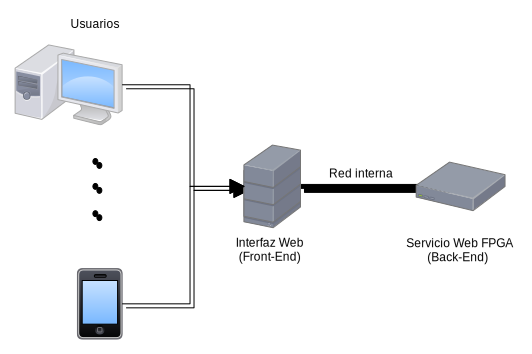
\includegraphics[width=0.7\textwidth,clip=true]{arquitectura}
  \caption{Arquitectura general de la aplicación.}
  \label{fig:arquitectura}
\end{figure}


\section{Back-End - Servicio Web FPGA\label{sec:dis:servicio_web_fpga}}

El componente \gls{back-end} se encarga de la interacción con la sonda de red (implementada en una \gls{FPGA}) y con el resto de partes involucradas en la reproducción y captura de tráfico de red.
Para ello, recibe peticiones \gls{HTTP} del \gls{front-end} (actuando en este caso como cliente), que se traducen en acciones sobre el sistema o en respuestas sobre el estado del mismo.
\begin{figure}[!htp]
  \centering
  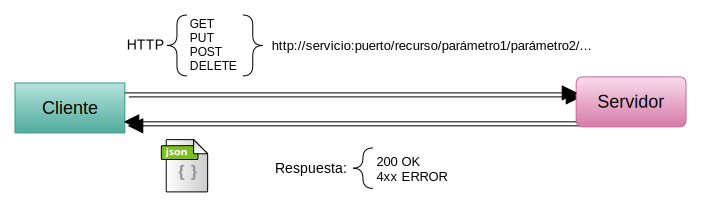
\includegraphics[width=0.95\textwidth,clip=true]{fpga_rest}
  \caption{Diagrama de flujo de un servicio \gls{REST}.}
  \label{fig:fpga_rest}
\end{figure}

La arquitectura de comunicación externa del \gls{back-end} se basa en el modelo de cliente-servidor \gls{REST} (ver Figura \ref{fig:fpga_rest}). Dentro de las directrices que marca este modelo, sólo se han considerado útiles para el problema dado un subconjunto de ellas:
\begin{itemize}
  \item El protocolo entre el cliente y el servidor debe ser sin estado: cada mensaje \gls{HTTP} tiene que contener toda la información necesaria para comprender la petición.
  \item Las operciones se aplican sobre recursos mediante llamadas a métodos \gls{HTTP}: \textit{GET} para obtener información sobre un recurso, \textit{POST}/\textit{PUT} para actualizarlos o crearlos y \textit{DELETE} para borrarlos.
  \item Cada recurso debe tener un identificador único (en este caso, una \gls{URL} única).
\end{itemize}

Se ha decidido no adoptar el resto de directrices \gls{REST} debido a que no encajaban dentro del modelo de funcionamiento de la aplicación.
Así, no se facilita el descubrimiento automático de recursos y métodos, ya que se ha considerado que no tiene sentido siendo éste un subsistema interno y no un componente público.
Por otra parte, no se permiten distintas representaciones de un mismo recurso, siendo \gls{JSON} la única representación utilizada.
No seguir estas directrices simplifica además la implementación del \gls{back-end}.

\begin{figure}[!htp]
  \centering
  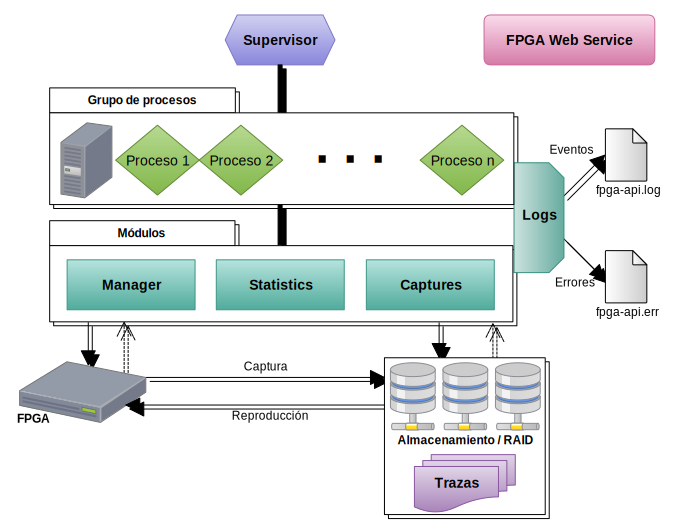
\includegraphics[width=0.95\textwidth,clip=true]{fpga}
  \caption{Arquitectura del \gls{servicioweb} \gls{FPGA}.}
  \label{fig:arquitectura_servicio}
\end{figure}

Internamente, \ref{fig:arquitectura_servicio}, 
Supervisor
1 párrafo Cluster de procesos para operaciones auxiliares, alta disponibilidad \ref{fig:arquitectura_servicio}
Logs
Módulos
Se distinguen por tanto, según su funcionalidad, tres módulos dentro del servicio web: gestión, captura y estadísticas.
\subsection{Gestión\label{ssec:dis:gestion}}

Este módulo tiene dos funciones principales: gestionar el estado de la sonda de red y gese encarga tanto de gestionar el estado de la sonda .
TODO: Gestión
  {Capturador,Reproductor}


\subsection{Capturas\label{ssec:dis:capturas}}

El módulo de capturas se encarga de todos los aspectos relacionados con las \glspl{traza} de tráfico de red.


detectar el formato interno de una \gls{traza}.

TODO: Capturas
  {Detección,Conversión,Renombrado,Borrado}


\subsection{Estadísticas\label{ssec:dis:estadisticas}}

estado, get
TODO: Estado/Estadísticas
  {Velocidad,Estado,RAID}


\section{Front-End - Interfaz web\label{sec:dis:interfaz_web}}

TODO: [Introducción] > sobre el framework, comunicación con el backend

Diseño responsive, visualmente atractiv. ventajas y diferencias vs adaptativo

Internacionalización

Introducción maquetas de las páginas principales

\subsection{Maquetas\label{ssec:dis:maquetas}}

\begin{figure}[!htp]
  \centering
  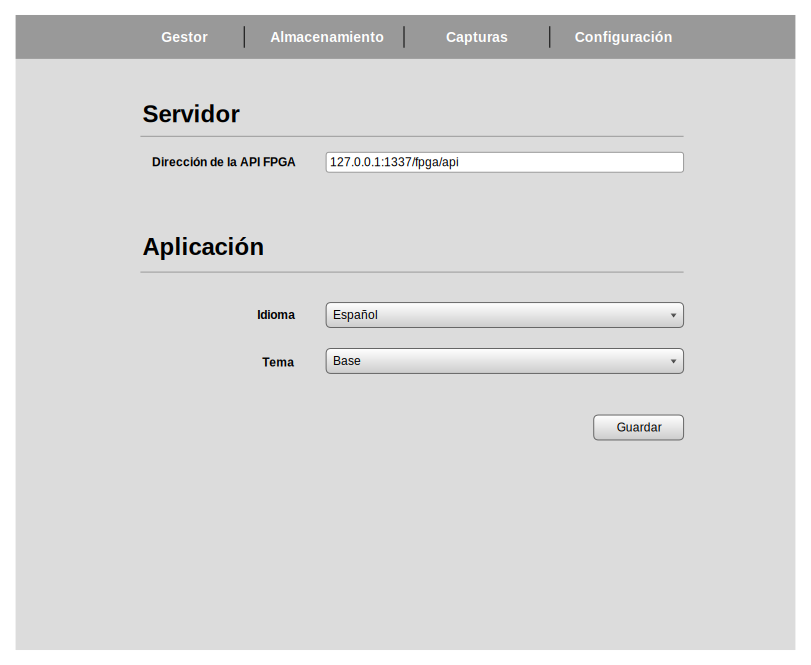
\includegraphics[width=0.95\textwidth,clip=true]{maquetas/maqueta_configuracion}
  \caption{Maqueta de la pantalla de configuración de la aplicación.}
  \label{fig:maqueta:configuracion}
\end{figure}

\begin{figure}[!htp]
  \centering
  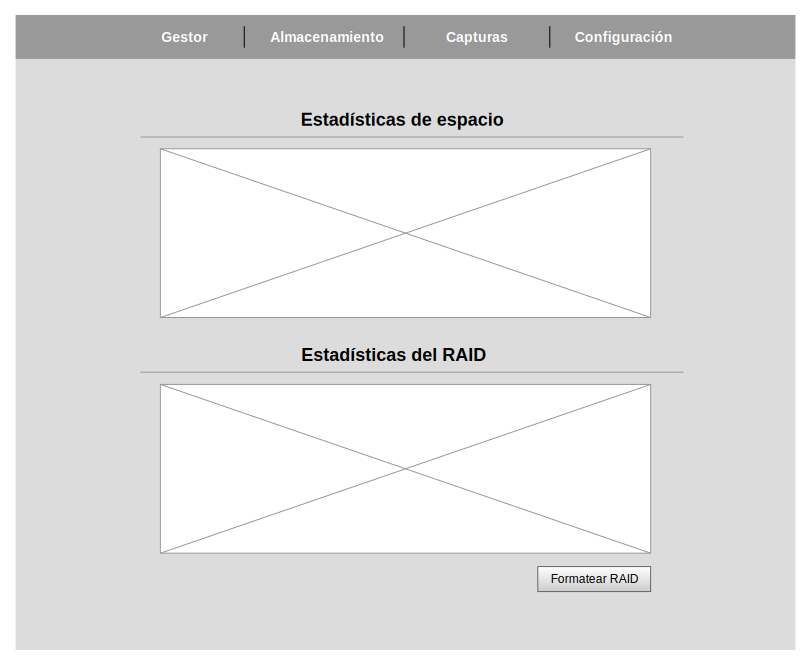
\includegraphics[width=0.95\textwidth,clip=true]{maquetas/maqueta_almacenamiento}
  \caption{Maqueta de la pantalla de almacenamiento.}
  \label{fig:maqueta:almacenamiento}
\end{figure}

\begin{figure}[!htp]
  \centering
  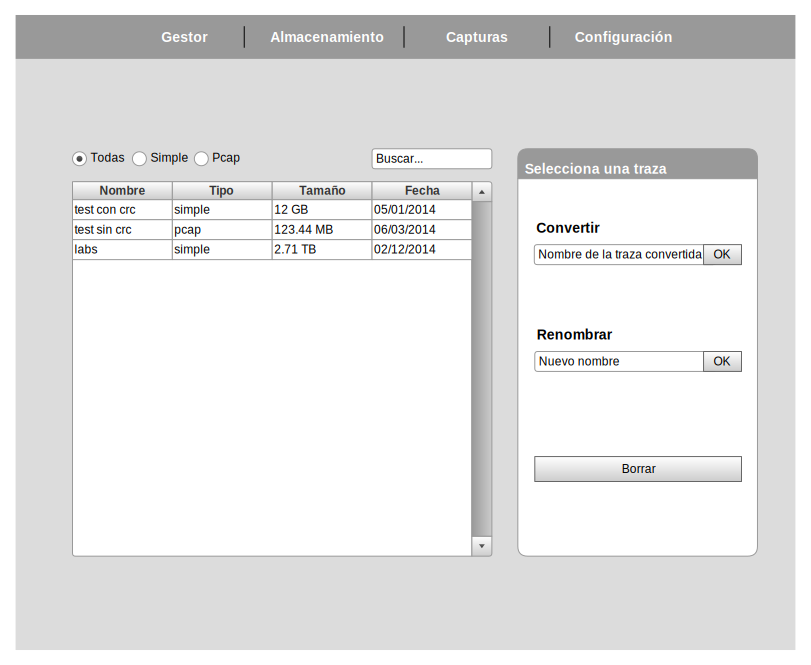
\includegraphics[width=0.95\textwidth,clip=true]{maquetas/maqueta_capturas}
  \caption{Maqueta de la pantalla de gestión de \glspl{traza}.}
  \label{fig:maqueta:capturas}
\end{figure}

\begin{figure}[!htp]
  \centering
  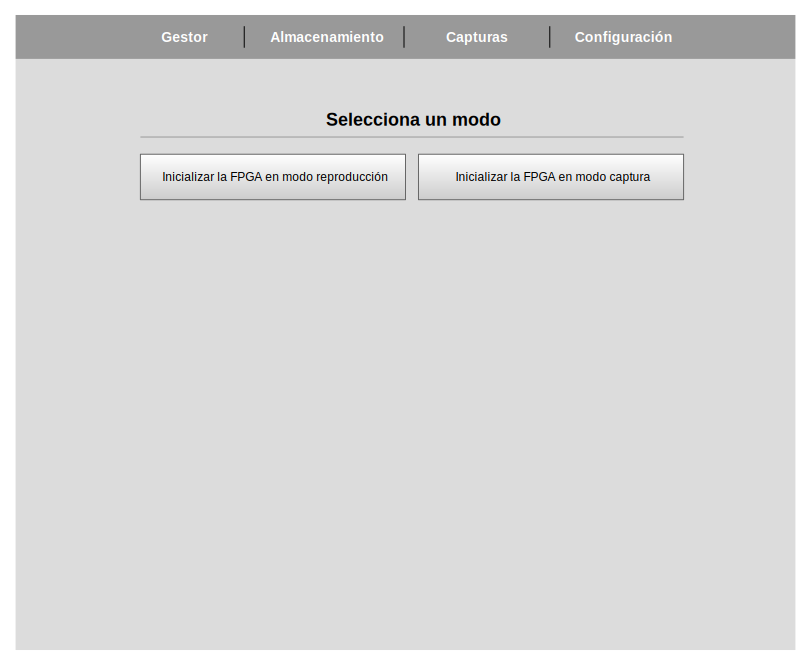
\includegraphics[width=0.95\textwidth,clip=true]{maquetas/maqueta_gestor_seleccion}
  \caption{Maqueta de la pantalla de gestión - selección de modo.}
  \label{fig:maqueta:gestor_seleccion}
\end{figure}

\begin{figure}[!htp]
  \centering
  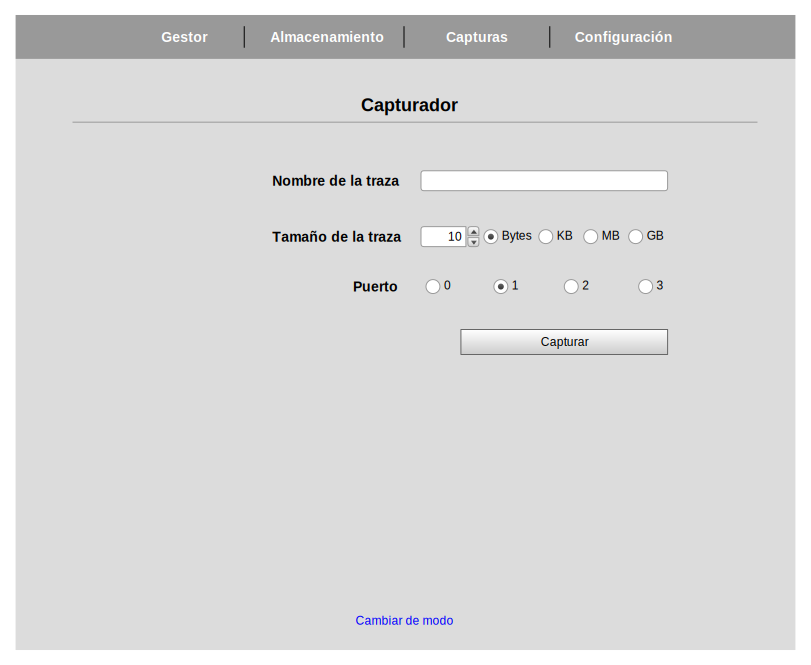
\includegraphics[width=0.95\textwidth,clip=true]{maquetas/maqueta_gestor_capturador}
  \caption{Maqueta de la pantalla de gestión - formulario para capturar.}
  \label{fig:maqueta:gestor_capturador}
\end{figure}

\begin{figure}[!htp]
  \centering
  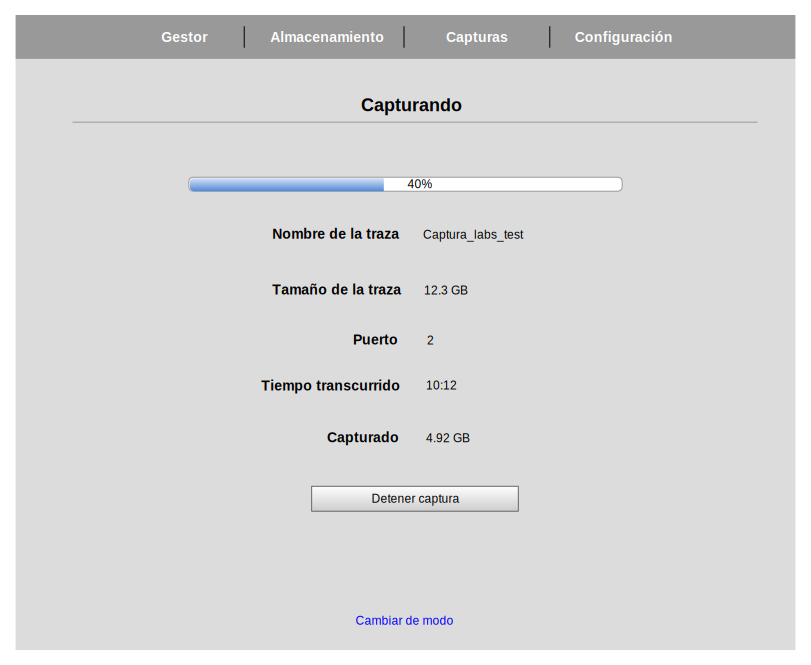
\includegraphics[width=0.95\textwidth,clip=true]{maquetas/maqueta_gestor_capturando}
  \caption{Maqueta de la pantalla de gestión - capturando.}
  \label{fig:maqueta:gestor_capturando}
\end{figure}

\begin{figure}[!htp]
  \centering
  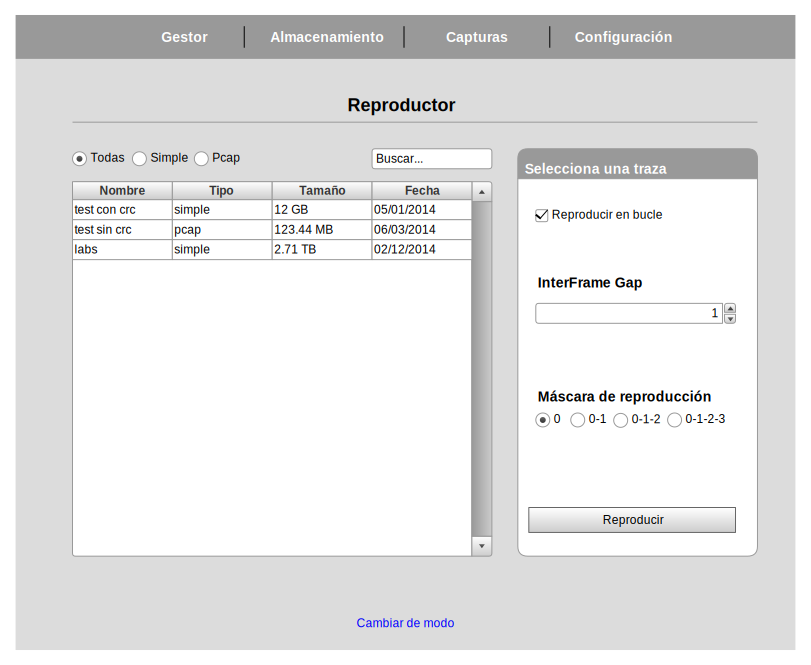
\includegraphics[width=\textwidth,clip=true]{maquetas/maqueta_gestor_reproductor}
  \caption{Maqueta de la pantalla de gestión - formulario para reproducir.}
  \label{fig:maqueta:gestor_reproductor}
\end{figure}

\begin{figure}[!htp]
  \centering
  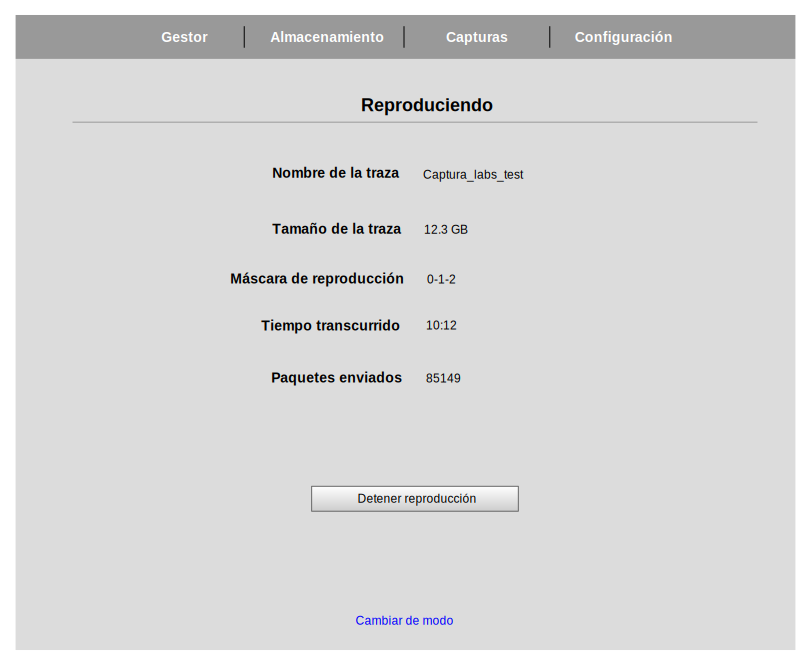
\includegraphics[width=\textwidth,clip=true]{maquetas/maqueta_gestor_reproduciendo}
  \caption{Maqueta de la pantalla de gestión - reproduciendo.}
  \label{fig:maqueta:gestor_reproduciendo}
\end{figure}